\documentclass[12pt,a4paper]{report}
\usepackage[utf8]{inputenc}
\usepackage{amsmath}
\usepackage{amsfonts}
\usepackage{amssymb}
\usepackage{makeidx}
\usepackage{graphicx}
\usepackage{cancel}
\usepackage{geometry}
\geometry{a4paper, top=10mm, left=10mm, right=10mm, bottom=20mm}
\author{Marius Ketterer}
\title{Praktikum Regelungstechnik 2 Abgabe Versuch 1 Digitale Übertragungsglieder}
\begin{document}

\maketitle
\tableofcontents

\chapter{Tiefpass 1.Ordnung}
\section{Aufstellen der Übertragungsfunktionen im s-Bereich inklusive Halteglied}
Aufstellen der Übertagungsfunktionen
\begin{equation}
G_{PT1}(s) = \frac{K}{1-Ts} 
\end{equation}
\begin{equation}
H(s) = \frac{1-e^{T_As}}{s}
\end{equation}
Transformieren in den Z-Bereich
\begin{equation}
G(z) = \mathcal{Z}\{H(s)*G_{PT1}(s)\} = \mathcal{Z}\left\{\frac{1-e^{T_As}* G_{PT1}(s)}{s}\right\}
\end{equation}

\begin{equation}
G(z) = \mathcal{Z}\left\{1-e^{T_As}*\frac{G_{PT1}(s)}{s}\right\} = (1-z^{-1})*\mathcal{Z}\left\{\frac{K}{s(1+Ts)}\right\}
\end{equation}

\begin{equation}
G(z) = (1-z^{-1})*\mathcal{Z}\left\{K\frac{\frac{1}{T}}{s(\frac{1}{T}+s)}\right\}
\end{equation}
\section{Transformation in den z-Bereich über Korrespondenztabelle}
Transformieren mit Hilfe der Korrespondenzentabelle(Nr.8)
\begin{equation}
G(z) = K*\cancel{(1-z^{-1})}*
\frac{(1-e^{-\frac{T_A}{T}})z^{-1}}
{\cancel{(1-z^{-1})}(1-e^{-\frac{T_A}{T}}z^{-1})}
\end{equation}
Daraus ergibt sich: 
\begin{equation}
G(z) = \frac{K*z^{-1}-e^{-\frac{T_A}{T}}z^{-1}}
{1-e^{-\frac{T_A}{T}}z^{-1}} 
\end{equation}
Einsetzen der Werte
\begin{equation}
K = 3; T = 4; T_A = 0,5s
\end{equation}
\begin{equation}
G(z) = \frac{3z^{-1}-e^{-\frac{0,5}{4}}z^{-1}}
{1-e^{-\frac{0,5}{4}}z^{-1}} = \frac{2,118z^{-1}}{1-0,882z^{-1}} = \frac{Y}{X}
\end{equation}
\begin{equation}
 Y- 0,882z^{-1}Y = 2,118z^{-1}X
\end{equation}
Nach $ Y $ aufgelöst ergibt das:
\begin{equation}
\Rightarrow Y = 2,118z^{-1}X - 0,882z^{-1}Y
\end{equation}
\section{Darstellung als Strukturplan}
\begin{figure}[ht]
	\centering
	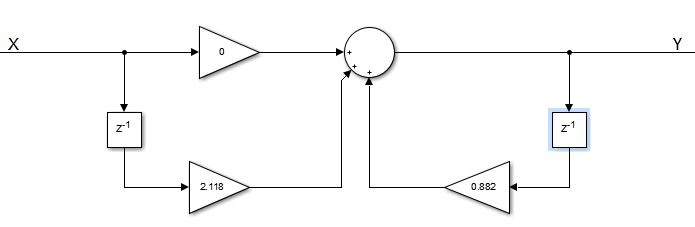
\includegraphics[width=0.8\linewidth]{marius/PT1}
	\caption{Struckturplan PT1}
	\label{fig:PT1}
\end{figure}

\chapter{Hochpass 1. Ordnung}
\section{Aufstellen der Übertragungsfunktionen im s-Bereich inklusive Halteglied}
Aufstellen der Übertagungsfunktionen

\begin{equation}
G_{DT1}(s) = \frac{Ks}{1-Ts} 
\end{equation}
\begin{equation}
H(s) = \frac{1-e^{T_As}}{s}
\end{equation}
Transformieren in den Z-Bereich
\begin{equation}
G(z) = \mathcal{Z}\{H(s)*G_{DT1}(s)\} = \mathcal{Z}\left\{\frac{1-e^{T_As}* G_{DT1}(s)}{s}\right\}
\end{equation}

\begin{equation}
G(z) = \mathcal{Z}\left\{1-e^{T_As}*\frac{G_{DT1}(s)}{s}\right\} = (1-z^{-1})*\mathcal{Z}\left\{\frac{K\cancel{s}}{\cancel{s}(1+Ts)}\right\} = (1-z^{-1})*\mathcal{Z}\left\{\frac{K}{(1+Ts)}\right\}
\end{equation}

\begin{equation}
G(z) = (1-z^{-1})*\mathcal{Z}\left\{\frac{K}{T}\frac{1}{s+\frac{1}{T}}\right\}
\end{equation}
\section{Transformation in den z-Bereich über Korrespondenztabelle}
Transformieren mit Hilfe der Korrespondenzentabelle(Nr.4)
\begin{equation}
G(z) = \frac{K}{T}*(1-z^{-1})*
\frac{1}
{1-e^{-\frac{T_A}{T}}z^{-1}}
\end{equation}
Daraus ergibt sich: 
\begin{equation}
G(z) = \frac{K-K*z^{-1}}
{T-e^{-\frac{T_A}{T}}z^{-1}*T} 
\end{equation}
Einsetzen der Werte
\begin{equation}
K = 3; T = 4; T_A = 0,5s
\end{equation}
\begin{equation}
G(z) = \frac{3-3*z^{-1}}
{4-e^{-\frac{0,5}{4}}z^{-1}*4} = \frac{3-3*z^{-1}}
{4-3,53z^{-1}} = \frac{Y}{X}
\end{equation}
\begin{equation}
4Y- 3,53z^{-1}Y = 3X -3z^{-1}X
\end{equation}
Nach $ Y $ aufgelöst ergibt das:
\begin{equation}
 4Y = 3X- 3z^{-1}X - 3,53z^{-1}Y
\end{equation}
\begin{equation}
\Rightarrow Y = \frac{3}{4}X- \frac{3}{4}z^{-1}X - 0,8825z^{-1}Y
\end{equation}
\section{Darstellung als Strukturplan}
\begin{figure}[ht]
	\centering
	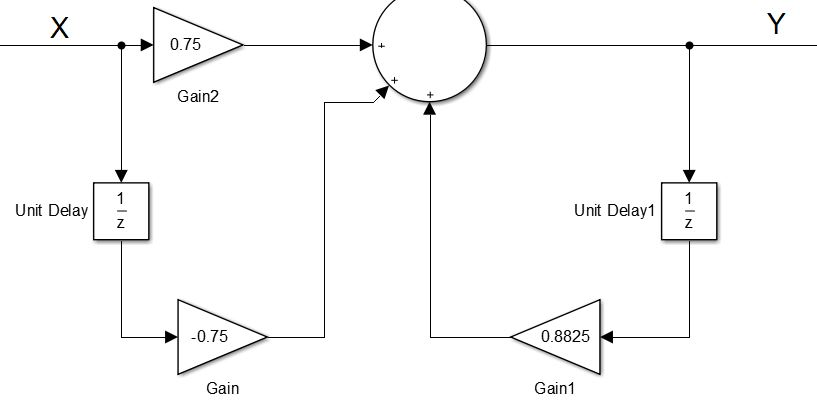
\includegraphics[width=0.8\linewidth]{marius/DT1}
	\caption{Struckturplan DT1}
	\label{fig:DT1}
\end{figure}


\end{document}